\chapter{系统功能需求分析与系统架构设计}

\section{系统功能需求}
文献X中表明,在一确定的CNN中,卷积的计算时间占据了至少85\%,因此若想制作一款CNN加速器,那么急需解决的问题就是如何加速图像的卷积计算。
卷积计算虽然参数相比于CNN中全连接层少,但其计算量非常大,而且通常为简单的乘加操作。
    \subsection{传统架构}
        \subsubsection{CPU}
        首先,CPU在深度学习计算中很重要,例如使用了16000颗CPU搭建的“Google Brain”网络,又比如1920颗CPU搭建的“AlphaGo”。如今,CPU依旧是主流深度学习平台的重要组成部分,
        但在深度学习领域,CPU在架构方面有着先天的不足,从芯片面积上看,Cache和Control单元占据了绝大部分面积,而用于计算的ALU面积却比较少;每颗核心都狠强大,但核心数量少。
        因此CPU重在数据调度,并不擅长大规模简单的运算。
        \subsubsection{GPU}
        反观GPU,虽然每颗核心都比较弱,只能完成简单的计算,但通常一个GPU都是上百上千个核心,芯片面积上用于计算的ALU单元占据了绝大部分,当所有核心都被调用起来,其运算能力远远大于CPU。
        同时,GPU普遍采用DDR5片上显存颗粒,更高的工作频率带来了更快的数据读写速度,而且总线带宽大。
    \subsection{异构的优势}
        目前做深度学习开发普遍采用CPU+GPU这种异构形式作为首要开发平台,既可以利用CPU强大的调度能力也可以利用GPU超快的计算速度,但这种模式是一种通用级的解决方法,应用在细分的专业领域边显的过于臃肿,不仅设备体积大,功耗也高。
        一般情况下,当模型训练完成后,需要利用模型进行推理计算,这部分不需要复杂的反向传播计算,若继续采用训练时的CPU+GPU平台,不仅造成资源浪费,量产时成本极高。
        因此针对推断,我们希望能找到一种低功耗、高性能的解决方案,因此使用FPGA和ASIC具有极大的优势。

        相比于通用的CPU+GPU的架构,CPU+FPGA/ASIC组成的异构平台具有更高的计算能效比,同时成本更低,十分适合当下嵌入式IoT领域对低功耗、高灵活性的需求。
        相比于受限于冯诺依曼架构的CPU/GPU,FPGA和ASIC在设计时可以通过多核心、流水线等技术充分发挥并行计算的特性,大大提高数据吞吐量。

\section{系统架构设计}
    针对本章第一节的需求,本文通过调研当前硬件加速方案,参考论文X的思想设计了一套针对CNN计算加速的方案。
    \begin{figure}[h]
        \centering
        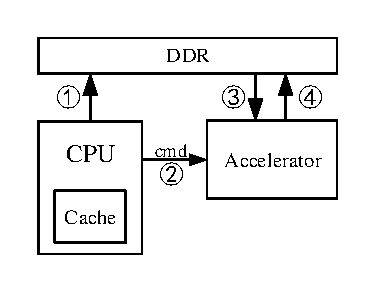
\includegraphics{../pdf/system.pdf}
        \caption{CNN加速系统架构示意图}
        \label{}
    \end{figure}

\section{开发环境}
    \subsection{HLS}
    HLS(High Level Synthesis)也既高层次综合技术,是Xilinx公司大力推广的一项FPGA开发技术。该技术使用C/C++作为开发语言,可以充分利用该语言中提供的数据结构进行FPGA开发。
    最终可以
    \subsection{HDL}
    \subsection{敏捷型开发}

\section{计算任务划分}

\section{基于行静止思想的卷积计算方法}

\section{本章小结}

% \subsection{二级节标题}

% \subsubsection{三级节标题}

% \paragraph{四级节标题}

% \subparagraph{五级节标题}

% \section{脚注}

% Lorem ipsum dolor sit amet, consectetur adipiscing elit, sed do eiusmod tempor
% incididunt ut labore et dolore magna aliqua. Ut enim ad minim veniam, quis
% nostrud exercitation ullamco laboris nisi ut aliquip ex ea commodo consequat.
% Duis aute irure dolor in reprehenderit in voluptate velit esse cillum dolore eu
% fugiat nulla pariatur. Excepteur sint occaecat cupidatat non proident, sunt in
% culpa qui officia deserunt mollit anim id est laborum.
% \footnote{This is a long long long long long long long long long long long long
% long long long long long long long long long long footnote.}
